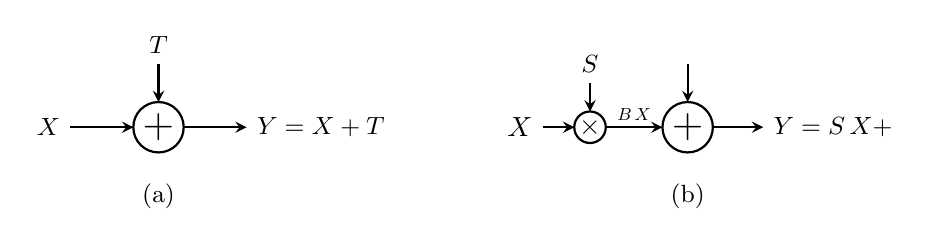
\begin{tikzpicture}[scale=.8]
\shorthandoff{>}
%
\begin{scope}
\draw[>=stealth,->,thick] (0,0) node[left]{\small $X$} --(1,0);
\draw[thick] (1.4,0) circle (.4);
\draw[>=stealth,->,thick] (1.4,1) node[above]{\small $T \N$} --(1.4,.4);
\node[align=center,scale=1.25] at (1.4,0){\large +};
\draw[>=stealth,->,thick] (1.8,0)--(2.8,0) node[right]{\small $Y = X + T \N$};
%
\end{scope}
%
\begin{scope}[xshift=7.5cm]
\draw[>=stealth,->,thick] (0,0) node[left]{$X$} --(.5,0);
\draw[thick] (.75,0) circle (.25);
\node[thick,align=center] at (.75,0){$\times$};
\draw[>=stealth,->,thick] (.75,.7) node[above]{\small $S$} --(.75,.25);
\draw[>=stealth,->,thick] (1,0)--(1.9,0);
\node[thick,align=center,scale=.7,above] at (1.45,0){\small $B \, X$};
\draw[thick] (2.3,0) circle (.4);
\draw[>=stealth,->,thick] (2.3,1) node[above]{\small $\N$} --(2.3,.4);
\node[align=center,scale=1.25] at (2.3,0){\large +};
\draw[>=stealth,->,thick] (2.7,0)--(3.5,0) node[right]{\small $Y = S \, X + \N$};
%
\end{scope}
\node at (1.4,-1.1){\small (a)};
\node at (9.8,-1.1){\small (b)};
\end{tikzpicture}
